% F089｜勾股整数数组的构造规律｜03_proof.tex
% 继承上传模板的 LaTeX 环境；当前条目的内容独立编写。
\clearpage
\begin{proofbox}
\textbf{\textcolor{CProof}{证明一（最快）：直接平方展开}}
\par\medskip
\begin{center}
% F089｜formula 原创简明教学示意图
\begin{tikzpicture}[>=stealth,scale=.9]
\node[draw,rounded corners,fill=teal!9] (a) at (0,0) {$m>n>0$};
\node[draw,rounded corners,fill=orange!10] (b) at (4.5,0) {$m^2-n^2,\ 2mn,\ m^2+n^2$};
\draw[->,thick] (a)--(b);
\node at (4.5,-1){\small 任取正整数 $m>n$，都会得到一组勾股数};
\end{tikzpicture}

\end{center}
\medskip
\[(m^2-n^2)^2+(2mn)^2\]$=m^4-2m^2n^2+n^4+4m^2n^2$ $=m^4+2m^2n^2+n^4=(m^2+n^2)^2$。因此总是勾股整数数组。
\end{proofbox}
\clearpage
\begin{proofbox}
\textbf{\textcolor{CProof}{证明二（最低门槛）：奇数公式}}
\par\medskip
\begin{center}
% F089｜odd 原创简明教学示意图
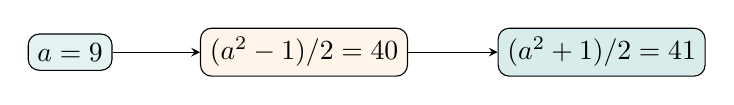
\begin{tikzpicture}[>=stealth,scale=.9]
\node[draw,fill=teal!10,rounded corners] (a) at (0,0){$a=9$};
\node[draw,fill=orange!8,rounded corners] (b) at (3.3,0){$(a^2-1)/2=40$};
\node[draw,fill=teal!15,rounded corners] (c) at (7.5,0){$(a^2+1)/2=41$};
\draw[->] (a)--(b);\draw[->] (b)--(c);
\end{tikzpicture}

\end{center}
\medskip
令奇数 $a\ge3$，取 $b=(a^2-1)/2,c=(a^2+1)/2$。两数相差1，因此 $c^2-b^2=(c-b)(c+b)=1\cdot a^2=a^2$，即 $a^2+b^2=c^2$。
\end{proofbox}
\clearpage
\begin{proofbox}
\textbf{\textcolor{CProof}{证明三（步骤最少）：偶数公式}}
\par\medskip
\begin{center}
% F089｜even 原创简明教学示意图
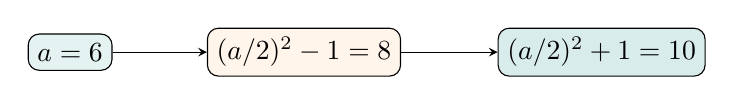
\begin{tikzpicture}[>=stealth,scale=.9]
\node[draw,fill=teal!10,rounded corners] (a) at (0,0){$a=6$};
\node[draw,fill=orange!8,rounded corners] (b) at (3.3,0){$(a/2)^2-1=8$};
\node[draw,fill=teal!15,rounded corners] (c) at (7.5,0){$(a/2)^2+1=10$};
\draw[->] (a)--(b);\draw[->] (b)--(c);
\end{tikzpicture}

\end{center}
\medskip
令 $a=2n$，其中 $n\ge2$；取 $b=n^2-1,c=n^2+1$，由平方差得 $c^2-b^2=(c-b)(c+b)=2\times2n^2=4n^2=a^2$。
\end{proofbox}
